\documentclass[conference]{IEEEtran}
\usepackage[pdftex]{graphicx}
\usepackage[cmex10]{amsmath}
\interdisplaylinepenalty=2500
\usepackage{array}
\usepackage{mdwmath}
\usepackage{mdwtab}
\usepackage{eqparbox}
\usepackage[font=footnotesize]{subfig}
\usepackage{fixltx2e}
\usepackage{url}
\hyphenation{}

% additional packages and utility commands

\usepackage{float}

\newcommand{\TODO}{\textbf{\color{red}TODO}}

% \usepackage{flushend}

% while preparing, linenumbers come in handy
\usepackage{lineno}
\setlength\linenumbersep{1mm}
\linenumbers

% until we settle on the final name ;-)
\usepackage{xspace}
\newcommand{\NAME}{id-foo\xspace}

% http://tex.stackexchange.com/questions/299/how-to-get-long-texttt-sections-to-break
\newcommand*\justify{%
  \fontdimen2\font=0.4em% interword space
  \fontdimen3\font=0.2em% interword stretch
  \fontdimen4\font=0.1em% interword shrink
  \fontdimen7\font=0.1em% extra space
  \hyphenchar\font=`\-% allowing hyphenation
}

% http://en.wikibooks.org/wiki/LaTeX/Customizing_LaTeX
\newcommand{\ttt}[1]{\texttt{\justify{#1}}}

\usepackage{algpseudocode}
% custom Let command
\newcommand*\Let[2]{\State #1 $\gets$ #2}
\renewcommand{\algorithmicforall}{\textbf{for each}}
\let\ForEach\ForAll

\usepackage{listings}

\usepackage{tikz}
\usetikzlibrary{positioning}
\usetikzlibrary{calc}
\usetikzlibrary{graphs}
\usetikzlibrary{trees}
\usetikzlibrary{arrows}

\usepackage{tikz-3dplot}

%!TEX root=paper.tex

% basics

\tikzset{
  box/.style            = { rectangle, minimum width=2cm, minimum height=1cm },
  border/.style         = { thick, draw=black },
  round/.style          = { rounded corners=3mm },
}

% system

\tikzset{
  artifact/.style       = { box, font=\ttfamily },
  support/.style        = { box, font=\itshape },
  user/.style           = { artifact, fill=black!15!white },
  dom/.style            = { support,  fill=black!30!white },
  platform/.style       = { support,  fill=black!55!white, text=white },
  native/.style         = { support,  fill=black!70!white, text=white },
  generated/.style      = { artifact, border, dashed },
  resource/.style       = { artifact, border },
  representation/.style = { support, border, round }
}

% UML

\tikzset{
  class/.style={
    box,
    border,
    text centered,
    text width=1.75cm
  },
  relation/.style       = { thick, draw=black, <-},
  subclass/.style       = { relation, >=open triangle 60 },
  aggregate/.style      = { relation, >=open diamond },
  composite/.style      = { relation, >=diamond },
  dependency/.style     = { relation, >=latex, -> }
}

\lstdefinelanguage{foo-lang}{
  emph={module,const,from,import,extend,with,after,do,function,@every,having,if,return},
  emphstyle={\textbf},
  morecomment=[l]{//},
  moredelim=[is][]{@@}{@@},       % temp solution to allow keywords without emph
  moredelim=[is][\emph]{!!}{!!}   % temp solution to hightlight #atoms
}


\usepackage[autostyle]{csquotes}

\usepackage{booktabs}
\usepackage{multirow}
\usepackage{stfloats}



\begin{document}

\title{
\NAME: A framework for \\
Efficient Intrusion Detection\\
in the Internet of Things
}

\author{\IEEEauthorblockN{Christophe Van Ginneken, Jef Maerien, Danny Hughes, 
Christophe Huygens, Wouter Joosen}%
\IEEEauthorblockA{iMinds-DistriNet, KU Leuven\\
3001 Leuven, Belgium\\
\{firstname.lastname\}@cs.kuleuven.be}}

\maketitle

\begin{abstract}

When intrusion prevention fails, intrusion detection serves as a second layer
of defense. It looks for patterns \& anomalies that can indicate malicious
behavior. But supporting an adequate set of intrusion detection algorithms
imposes significant overhead on resource-restricted devices such as those
targeting the Internet of Things. Fusion of the algorithms, to optimize sharing
of resources, can alleviate this, yet, proves to be time-consuming, repetitive
and error-prone. To address this problem we introduce \NAME, a framework for
the development of efficient intrusion detection systems. It consists of a
domain specific language, to formally describe intrusion detection algorithms
on a functional level, and a code generator to produce more optimally organized
source code. A side-by-side comparison shows that generated code reduces memory
footprint, message passing overhead and execution time in comparison to a
straightforward sequential implementation of the same algorithms.

\end{abstract}

\section{Introduction}

% context

% IoT + threat

The internet of things (IoT) holds a great potential to positively influence
our daily work and life through domotics, assisted living, e-health and
enhanced learning \cite{atzori2010internet}. But with this potential the IoT
also presents a significant threat: by opening our smart homes and personal
data to all these interconnected devices, we also open them to everyone who is
able to break the virtual locks (i.e.\ passwords, encryption keys,\dots) that
protect them. IoT devices typically have limited batteries, processing power
and memory. These properties make it hard to add any additional service,
including security.

% classic networks: fw and central ids

In classic networks, firewalls focus on the outer perimeter of the network,
filtering unwanted packets and protecting the entire internal network. But
attacks on flaws in services can pass unnoticed. This is where intrusion
detection (ID) steps in: an ID probe monitors all traffic that passes through
the firewall, looking for patterns and optionally, after detecting a malicious
pattern, alerting the firewall \cite{denning1987intrusion}.

% local ids -> localize -> limited resources

In wireless networks of resource constraint devices, which make up an
significant part of the IoT, it is not possible to have this single point in
the network that can oversee all traffic \cite{mishra2004intrusion}. Every
device has to implement its own lines of defense. But making the intrusion
detection system (IDS) a local service on each device requires local resources,
which are a scarce commodity for IoT devices.

Attackers have access to a large set of possible attack vectors
\cite{aschenbruck2012security}, ranging from the wireless network, over the
medium access control and routing, up to the device itself. Each level presents
different opportunities to manipulate data, eavesdrop, perform a form of denial
of service or access the network in a legitimate way. For each of these attacks
an algorithm needs to look for patterns or anomalies. An IDS for IoT devices
therefore requires a large number of implemented algorithms for an adequate
coverage.

% gap analysis

Current developments in ID focus on programming frameworks to structure the
implementation of algorithms \cite{valero2012di} and offer the required basic
functional components to implement them \cite{krontiris2008lidea}. The first
aspect that is missing, is that they don't offer a way to optimize the usage of
resources. A solution that supports the integration of multiple algorithms on
IoT devices needs to consider the impact on their resources and avoid
accumulating their impact.

A second omission is support for systematic reuse to create different
configurations for different devices, both in hard- and software. Addressing
this in a transparent and automated way is important for any kind of
development in this area.

% scientific contribution

% 1. framework: language + code generator

The first contribution of this paper is a framework that enables the formal
description of ID algorithms on a functional level. An automated code
generation process produces corresponding source code, for a given platform and
configuration. This way, the framework addresses the heterogeneous nature of
both the IoT and ID algorithms.

% 2. FCF to optimise

The second contribution introduces functional code fusion (FCF) as a generation
paradigm to solve the problem of hard to reuse and combine ID algorithms. FCF
identifies common data and functions, and organizes code to eliminate redundant
iterations, tests and computations. Results show improved memory usage,
execution time and usage of the wireless radio, reducing energy consumption.

% structure

The remainder of this paper proceeds as follows: section \ref{classification}
analyses and classifies ID algorithms. Section \ref{pattern} looks for patterns
in the implementation of these classes and details the ideas behind FCF\@.
Section \ref{design} describes the design we applied to construct the
framework, its domain specific language (DSL) and code generator. Section
\ref{evaluation} evaluates an implementation of the framework. Section
\ref{related} explores related work in the field of DSLs for ID and code
generation for the IoT\@. Finally, section \ref{conclusion} summarizes our
findings, draws conclusions and identifies topics for future work.

\section{A Classification of ID Algorithms}
\label{classification}

Two aspects, currently missing from ID frameworks, that \NAME wants to cover
are optimization of resources and support for systematic reuse. This section
uses a classification to define the scope of \NAME, detailing which types of
algorithms are good candidates for the proposed approach.

Research into ID in wireless networks typically focuses on two major topics:
the devices as single entities and the network as a group of such devices. Both
are important: a group cannot make a decision without members that detect
malicious behavior and a group-based decision is often needed because nodes in
the network can miss certain events that could reveal intrusions. In a wireless
network, where not all participants are within each others' radio range, nodes
typically only have a partial view on the entire network. This prohibits them
to observe potentially crucial events in distant parts of the network. The fact
that resource constraint devices typically apply duty cycling to lower their
energy consumption, further increases this problem, introducing periods of time
where they even don't see local events.

This leads to two complementary classes of ID activities: local intrusion
detection and cooperative decision making.

\subsection{Local Intrusion Detection}
\label{detection}

There are different ways to construct a taxonomy for intrusion detection, but
common themes do appear. According to \cite{mishra2004intrusion} and
\cite{ioannis2007towards} there are three major categories: anomaly detection,
signature or misuse detection, and specification-based detection. In
\cite{alrajeh2013intrusion} the authors agree with this typology and add the
notion of hybrid intrusion detection systems and cross layer intrusion
detection systems as recent advances in research. Although these additional
categories seem promising, the authors admit that the impact on
resource-constrained devices will be too much. We therefore focus on the three
categories agreed upon by most sources.

\begin{LaTeXdescription}
  
  \item[Anomaly detection] considers a baseline profile and evaluates all
  activity according to this profile. It tries to flag aberrant behavior as a
  possible intrusion. The baseline profile can evolve over time, especially in
  wireless and mobile environments. Single events should therefore not result
  in absolute decisions.
  
  \item[Signature or misuse detection] starts with known patterns of attacks.
  It tries to find evidence for intrusions in the actions of and communication
  with a device. Because attacks often use valid ways to communicate with
  services on the devices, this approach can produce false positives.
  
  \item[Specification-based detection] uses constraints that describe the
  correct behavior of the system. Although that this approach can detect
  previously unknown attacks, it can sometimes not detect specific attacks that
  anomaly or misuse detection can.
  
\end{LaTeXdescription}

\subsection{Cooperative Decision Making}
\label{coorperative}

These taxonomies focus on the act of detecting intrusions themselves. In a
distributed environment, communication between participants may be even more
important.

Because not all devices are always actively participating in the network, they
can miss clues that would otherwise lead them to detect intrusions. It is
hardly impossible for a single device to detect a complex attack by itself.
Therefore a second important research topic consists of cooperative algorithms
to combine information from single identities into a group-based decision about
alleged intrusions. We identify two ways to construct cooperative decision
making and focus on the way participants exchange information: broadcasting and
interactive.

\begin{LaTeXdescription}

  \item[Broadcasting] can sometimes allow to implement a distributed,
  cooperative algorithm locally. The reputation-based detection algorithm
  introduced in \cite{ganeriwal2008reputation} illustrates this, based on the
  same principle of a watchdog also found in \cite{mishra2004intrusion}. Using
  this algorithm, nodes can exchange information about the reputation of other
  nodes, solely with broadcasts. Combining this information allows them to
  decide about their trust in a given node, based on more than their own, often
  partial, observations alone.

  \item[Interactive] communication allows algorithms to exchange information to
  reach a consensus. In \cite{krontiris2009cooperative}, the authors first
  present a theoretical foundation to analyze cooperative algorithms. Given
  these foundations they continue to present an algorithm consisting of 5
  phases. It essentially implements a voting system-based on the Guy Fawkes
  protocol \cite{anderson1998new} to identify an intruder. It enables the
  exchange of suspected intruder information and allows distributed
  authentication of those \emph{votes}. Based on these authenticated votes, the
  participants can make a distributed decision about the jointly identified
  intruder.

\end{LaTeXdescription}

\subsection{Properties and Scope of \NAME}
\label{scope}

Algorithms that fit this classification are typically platform independent.
They analyze network messages, looking for patterns that can reveal intrusions
and deal with the same information: other nodes in the network. To be able to
formally describe ID algorithms and target the heterogeneous IoT, \NAME
requires ID algorithms to expose these properties.

A class of ID algorithms that does not have these properties is software
attestation \cite{seshadri2008sake}. It enables exchanging information about
the software that is running on a device and identifying devices with modified
content. These algorithms are highly platform dependent and have no data in
common with other algorithms, as they look for the effects of an intrusion, not
the intruder itself.

Figure \ref{fig:classification} visually summarizes the dual classification and
scope of \NAME.

\begin{figure}[ht]
  \centering
  \scalebox{.85}{
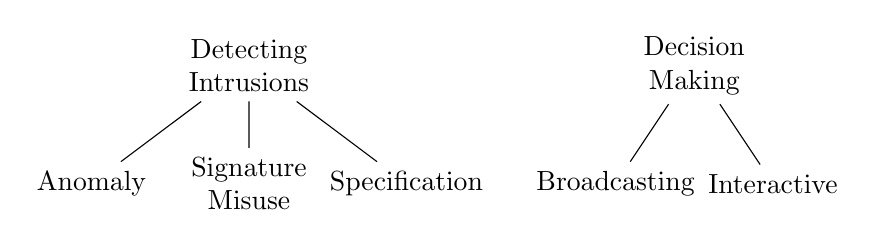
\begin{tikzpicture}[
  sibling distance=20mm,node distance=40mm
  ]
  \node (detection)             [align=center] {Detecting\\Intrusions}
    child {node (anomaly)       [align=center] {Anomaly}}
    child {node (signature)     [align=center] {Signature\\Misuse}}
    child {node (specification) [align=center] {Specification}};
  \node (decision)              [align=center,right=of detection] {Decision\\Making}
    child {node (broadcasting)  [align=center] {Broadcasting}}
    child {node (interactive)   [align=center] {Interactive}};
\end{tikzpicture}
}
  \caption{Classification of ID Algorithms}
  \label{fig:classification}
\end{figure}

\section{A Design Pattern for ID Algorithms}
\label{pattern}

Given this classification, we now introduce a design pattern that identifies
common functional aspects of these algorithms. It will allow us to define a
strategy for optimizing the combination of these algorithms. From the
classification and a survey of algorithms, we extract two activities common to
most algorithms: the inspection of network traffic and the evaluation of
thresholds.

Network traffic is the carrier along which malicious payloads reach a device
directly. Indirectly a device can also detect aberrant patterns of
communication by other devices, as a result of a successful attack.

Not all algorithms can decide if an attack is real or not, based on a single
event. Signature and misuse detection can in some cases, but anomaly detection
typically deals with some level of uncertainty. Also, in distributed situations
it is impossible to fully trust any neighboring device. In these situations one
has to rely on statistics and thresholds to decide when to drop trust in a
given device.

But simply checking a threshold after updating some counter, is not a good
strategy. A simple example is that of a watchdog \cite{mishra2004intrusion},
observing the actions of other devices. There are valid reasons why a device
can miss a theoretical window in which one expects activity, i.e.\ the wireless
network being the most predominantly unreliable component. Directly reacting on
a basic threshold can result in false positives. A way to overcome this is to
decouple the detection of problems and the decision what to do about them.

This decoupling of detection and decision is the core of the design pattern for
ID algorithms. Listing \ref{alg:id-algo-pattern} presents the design pattern in
pseudo-code.

\begin{figure}[ht]
\captionof{lstlisting}{ID Algorithm Pattern\label{alg:id-algo-pattern}}
\begin{algorithmic}[1]
  \Require{nodes, global storage for information about nodes}
  \Function{process\_message}{$msg$}
    \ForEach{$byte \in msg$} \label{alg:id-algo-pattern-loop1}
     \State \dots \Comment{analyze byte-sequences}
    \EndFor
    \Let{$nodes_x$}{value}  \Comment{optionally update node info}
    \State \Call{send}{$nodes_y$, ``info''} \Comment{optionally exchange info} \label{alg:id-algo-pattern-send1}
  \EndFunction
  \State
  \Function{do\_housekeeping}{}
    \ForEach{$node \in nodes$} \label{alg:id-algo-pattern-loop2} \label{alg:id-algo-pattern-common-data}
      \If{$node > \dots$} \Comment{validate recorded value}
        \State \dots \Comment{take actions}
        \State \Call{send}{$node$, ``info''} \Comment{communicate} \label{alg:id-algo-pattern-send2}
      \EndIf
    \EndFor
  \EndFunction
  \State
\end{algorithmic}
\end{figure}

We now extend the scope of the design pattern, to include its application in
the context of multiple algorithms. When implementing different algorithms, a
pattern such as described in listing \ref{alg:id-algo-application} will
typically appear.

\begin{figure}[ht]
\captionof{lstlisting}{Application pattern of multiple ID algorithms\label{alg:id-algo-application}}
\begin{algorithmic}[1]
  \Let{$msg$}{$network$} \Comment{all observed messages}
  \ForEach{$algorithm \in algorithms$}
    \State \Call{algorithm.progress\_message}{msg}
  \EndFor
  \State \dots
  \Comment{at a given interval}
  \ForEach{$algorithm \in algorithms$}
    \State \Call{algorithm.do\_housekeeping}{}
  \EndFor
\end{algorithmic}
\end{figure}

The pattern calls the different, linked implementations in a sequential way in
two situations: first, when the device observes new messages on the network
and, secondly, at a regular interval to allow for internal housekeeping, such
as threshold evaluation.

\subsection{Inherent Problems}
\label{pattern-problems}

These patterns can now help in identifing the problem areas that tend to result
in suboptimal code when combining multiple ID algorithms. Two issues arise from
the nested loops that originate from the combination of the ID algorithm
pattern and the application pattern: loops and common data. A third issue is
the use of the network.

\begin{LaTeXdescription}

  \item[Loops] by themselves are not a problem, but different loops, that
  perform the same operations in sequence, can incur an overhead. An example
  from the ID algorithm pattern is the handling of messages: each algorithm
  parses each observed message on the network, processing the same byte stream,
  performing comparable operations to find similar patterns.

  \item[Common data] cross-cuts the different algorithms, that have to store
  information about nodes within its own scope. This results in a lot of
  duplicated information in memory.

  \item[The network] allows algorithms to operate on a distributed scale. But
  scattered calls to the \ttt{SEND} function cause multiple accesses to the
  wireless radio, keeping it active and energy consuming more than strictly
  needed.

\end{LaTeXdescription}

\bigskip
Two operational aspects are orthogonal to these problems and amplify them:

\begin{LaTeXdescription}
  
  \item[Reimplementing] the algorithms manually to eliminate these issues is
  not a one-time cost. For example due to the release of a new version of an
  algorithm, or simply a reselection of algorithms due to a changing risk
  analysis. Also, changing, or simply implementing the algorithms from scratch,
  holds the risk of making mistakes.

  \item[The heterogeneity of IoT devices] results in different software stacks,
  each with for example their own network API\@. This also explains why there
  are no implementations readily available to developers: there is no single
  platform to target for researchers.

\end{LaTeXdescription}

\section{Design}
\label{design}

The previous sections identified loops, common data and the network as three
important code-level problems. These problems are inherent to ID algorithms.
But at the same time they conflict with their target environment, the IoT\@.
\NAME provides a framework to efficiently implement an IDS for the IoT and
offers a solution for the identified problems. It consists of a DSL, source
code generator and software library. Figure \ref{fig:design} visualises the
overall design.

\begin{figure}[ht]
  \centering
  \scalebox{.85}{
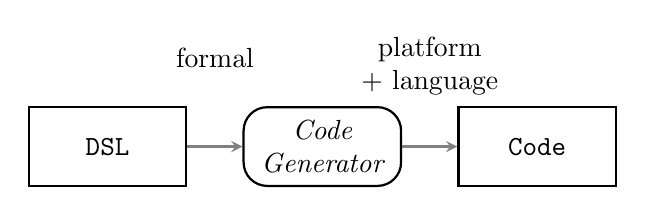
\begin{tikzpicture}[
  node distance=7mm,
  ,>=stealth,thick,black!50,text=black,
  every new ->/.style={shorten >=1pt}
]
  \node (dsl)  [resource]                                 {DSL};
  \node (cg)   [representation,right=of dsl,align=center] {Code\\Generator};
  \node (code) [resource,right=of cg]                     {Code};

  \draw [->] (dsl) -> (cg)   node [midway,above=25pt]              {formal};
  \draw [->] (cg)  -> (code) node [midway,above=15pt,align=center] {platform\\ + language};

\end{tikzpicture}
}
\caption{Overall Design}
\label{fig:design}
\end{figure}

The DSL enables researchers to formally describe ID algorithms, without
focusing on any specific language or platform. A code generator can combine
such formal descriptions, avoiding the identified problems concerning loops,
common data and network access. It can also target different languages and
platforms, while reusing a software library that provides services including
parsing, network access wrapping,\dots

A DSL and code generator defines a development strategy. This implies choices
with respect to flexibility, update cost and development effort. We will first
position \NAME and motivate its design with respect to these trade offs.
Second, we will look at the principal design components of the DSL and how it
deals with loops and common data. Third, we discuss the structure of the code
generator and introduce its software library, that offers a way to deal with
the network access issue.

\subsection{\NAME as a Development Strategy}
\label{positioning}

Figure \ref{fig:positioning} shows a classification of possible development
strategies for projects involving wireless devices.

\newcommand{\ball}[5][above,yshift=+5pt]{
\tdplottransformmainscreen{#2}{#3}{#4}
\shadedraw[tdplot_screen_coords, ball color=lightgray,draw=lightgray,shading angle=-90]
  (\tdplotresx,\tdplotresy) circle (0.20)
  node[text=gray,font=\footnotesize,#1]{#5};
}

\begin{figure}[ht]
  \centering
  \scalebox{.85}{
\tdplotsetmaincoords{110}{-10}
\begin{tikzpicture}[scale=1,tdplot_main_coords]
  % axis
  \draw[thick,->] (0,0,0) -- (7,0,0) node[anchor=north east,xshift=10mm]{$flexibility$};
  \draw[thick,->] (0,0,0) -- (0,7,0) node[anchor=north west]{$update\ cost$};
  \draw[thick,->] (0,0,0) -- (0,0,4) node[anchor=south]{$development$};
  % points
  \coordinate (O)        at (0,0,0);
  \coordinate (ideal)    at (6,0,0);
  \coordinate (vm)       at (2,2,2);
  \coordinate (modular)  at (4,4,4);
  \coordinate (reconfig) at (4,2,4);
  \coordinate (full)     at (6,6,4);
  \coordinate (cg)       at (6,4,2.5);
  % "lines"
  \draw[dashed] (2,0,0)    -- (2,2,0) -- (0,2,0);
  \draw[dashed] (4,0,0)    -- (4,4,0) -- (0,4,0);
  \draw[dashed] (6,0,0)    -- (6,6,0) -- (0,6,0);
  \draw[dashed] (vm)       -- (2,2,0);
  \draw[dashed] (modular)  -- (4,4,0);
  \draw[dashed] (full)     -- (6,6,0);
  \draw[dashed] (reconfig) -- (4,2,0);
  \draw[dashed] (cg)       -- (6,4,0);
  % "balls"
  \ball{6}{0}{0}{ideal}
  \ball{2}{2}{2}{virtual machine}
  \ball[left,xshift=-5pt]{4}{4}{4}{\shortstack{modular\\native image}}
  \ball{4}{2}{4}{\shortstack{reconfigurable\\virtual machine}}
  \ball[right,xshift=+5pt,yshift=+5pt]{6}{6}{4}{full native image}
  %\ball[right,xshift=+5pt,text=black]{6}{4.5}{3}{code generation};
  % 5. cg
  \tdplottransformmainscreen{6}{4}{2.5}
  \shadedraw[tdplot_screen_coords, ball color=gray,draw=black,shading angle=-90]
    (\tdplotresx,\tdplotresy) circle (0.20)
    node[right,xshift=+5pt,text=black,align=center,font=\footnotesize]{code generation\\+ functional code fusion};
  % "box around our solution" ;-)
  \tdplottransformmainscreen{0}{0}{0}
  \draw[tdplot_screen_coords] (4.95,1) rectangle (8.5,0.25);

\end{tikzpicture}
}
\caption{Classification of Development Strategies for Wireless Devices (based on \cite{sadilek2007energy})}
\label{fig:positioning}
\end{figure}

Three properties can classify development strategies \cite{sadilek2007energy}:
flexibility, update cost and development effort.

\begin{LaTeXdescription}

  \item[Flexibility] is a measure for the number of applications one can deploy
  on a device without physical access.
  
  \item[Update cost] is equivalent to the energy required to deploy a new
  version of an application on a device.
  
  \item[Development effort] covers the time to write, test and deploy an
  application.

\end{LaTeXdescription}

The \emph{ideal} situation is that were one ends up with a maximal flexibility
and no update nor development cost.

If we consider the trade off between flexibility and update cost, we can
distinguish two extremes: \emph{virtual machines} and \emph{full native
images}. Virtual machines allow for small updates due to their concise byte
code, but their instruction set and predefined capabilities restrict them at
the same time. A full native image on the other hand has unlimited flexibility,
but requires transfer of a larger image over the network.

Two intermediate alternatives are possible: \emph{modular native image} and
\emph{reconfigurable virtual machines}. Modular native images allow changes on
module level, limiting the update size, but the framework to support it is
static and limits the possibilities. Reconfigurable virtual machines take this
same approach, but apply it to virtual machines, allowing to \emph{upgrade} the
instruction set of the virtual machine.

\NAME starts from the full native image, allowing full flexibility, and aims to
reduce both the update and development cost. Firstly, by applying functional
code fusion, \NAME optimizes the code organization, which has a positive effect
on the code size and hence also on the update cost. Secondly, by enabling reuse
on a functional level and automating the writing phase, the development cost is
also lowered.

\subsection{\NAME as a Domain Specific Language}
\label{dsl-design}

It's important to remember that a DSL is merely a \emph{thin veneer over a
(semantic) model} \cite{fowler2010domain}. Its sole purpose should be
populating the model. \NAME's DSL and model focuses on avoiding constructions
that result in problems concerning loops, common data and the use of the
network. To do this, \NAME uses an event-based approach to defining
functionality.

\subsubsection{Loops}

Loops are a major contributor to the problem of algorithm fusibility. Loops in
program code are technical constructs and in fact often hide the intended
functionality.

The example of parsing network messages illustrates this. Each algorithm deals
with parsing in the same way: loop over the bytes in the payload and look for a
pattern that identifies what the algorithm is looking for. This is in fact a
technical implementation choice. The underlying functional goal is to react
when such a pattern is present in a message. The loop has \emph{activated} this
functionality, but the real goal is to \emph{passively} react on an event, not
\emph{actively} look for it. Event handling therefore can transform
constructions with loops to their functional meaning, allowing identification
and fusion of common functionality.

The same goes for actively polling some variable until it reaches a certain
threshold. When transformed to a reaction to an event, it eliminates the need
for a technical loop-construction.

\subsubsection{The Nodes Domain}

All algorithms deal with information about neighboring devices. To centralize
this information \NAME provides a unified \ttt{nodes} concept as part of its
DSL and exposes it as an object to the implementer.

Algorithms can extend nodes with their own properties. This way only one
instance for every known device will be present in memory. Finally, nodes can
define a scope to execute a function in. This way, nodes also offer a way to
iterate all known devices, again without the need for a loop.

\subsubsection{Unified Messaging}
\label{dsl-unified-msg}

Access to the network, scattered around an algorithm, causes the wireless radio
to be more active than needed. Delaying the sending of messages and grouping
them, can lower this overhead.

Sending and receiving of network messages is tightly integrated with the
previously mentioned concepts of event handling and the nodes domain. An
underlying software framework will handle all interaction with the network,
triggering functions by means of events when parsing new messages and exposing
an API to send messages through the nodes domain. This approach gives the
framework complete control over communication, allowing optimized marshaling,
grouping,\dots

\subsubsection{An Example}

Listing \ref{lst:watchdog} illustrates some of the features mentioned above,
using a small but representative example of an algorithm: a
watchdog \cite{mishra2004intrusion}. Like a heartbeat, nodes can broadcast a
message at a regular interval, allowing other nodes to monitor its
availability. Missing heartbeats could indicate problems, such as physical
capturing of a device.

\lstinputlisting[
  language=foo-lang,
  float,
  basicstyle=\footnotesize\ttfamily\color{black},
  label=lst:watchdog,
  caption=Watchdog in \NAME
]{src/watchdog.foo}

\subsection{\NAME as a Code Generator}
\label{code-generator-design}

To convert the DSL-based ID algorithms into production-ready code, we apply
code generation techniques. Although different approaches here are applicable,
like template-based text expansion, XSLT transformations or CodeDom
\cite{dollard2004code}, we believe that the functional transformations require
a richer model.

A semantic model \cite{fowler2010domain}, tied closely to the DSL itself, can
fulfill this role. Semantic transformations evolve the model into a
syntax-oriented model, comparable to the idea of CodeDom. From there on,
syntactic transformations an emit source code. Figure \ref{fig:code-generation}
shows the process that \NAME implements.

\begin{figure}[ht]
  \centering
  \scalebox{.85}{
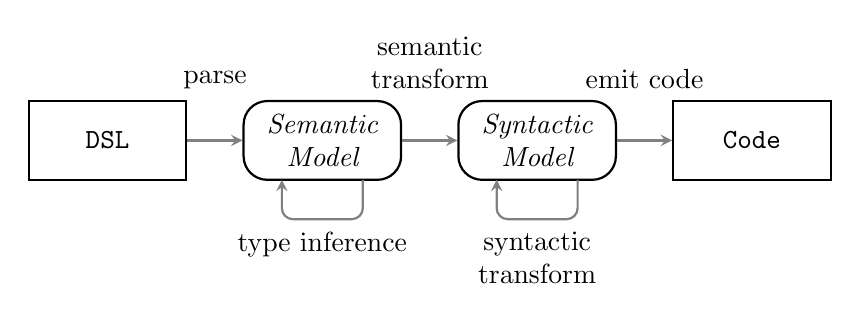
\begin{tikzpicture}[
  node distance=7mm,
  ,>=stealth,thick,black!50,text=black,
  every new ->/.style={shorten >=1pt}
]
  \node (dsl)  [resource]                                 {DSL};
  \node (sm)   [representation,right=of dsl,align=center] {Semantic\\Model};
  \node (cm)   [representation,right=of sm,align=center]  {Syntactic\\Model};
  \node (code) [resource,right=of cm]        {Code};


  \draw [->] (dsl) -> (sm)   node [midway,above=15pt]              {parse};
  \draw [->] (sm)  -> (cm)   node [midway,above=15pt,align=center] {semantic\\transform};
  \draw [->] (cm)  -> (code) node [midway,above=15pt]              {emit code};

  \draw [rounded corners,->]
        ($ (sm.east) - (5mm,5mm) $)
        -- ++(0,-.5)
        -| ($ (sm.west) + (5mm,-5mm) $)
           node [near start, below=1pt] {type inference};

  \draw [rounded corners,->]
        ($ (cm.east) - (5mm,5mm) $)
        -- ++(0,-.5)
        -| ($ (cm.west) + (5mm,-5mm) $)
           node [near start, below=1pt,align=center] {syntactic\\transform};

\end{tikzpicture}
}
\caption{Overview of \NAME's code generation process}
\label{fig:code-generation}
\end{figure}

After parsing the DSL, it's imported into a semantic model. The minimal type
information present in the initial model allows inferring of the remaining
types. Through a series of semantic transformations, the model evolves from the
functional to a more technical syntactic model. This model is comparable to a
rich abstract syntax tree (AST) with an extensive set of language constructs.
Syntactic transformations now lower this level of expressiveness according to
the desired platform and language. In the end the syntactic model can be
directly emitted to the target language.

\subsubsection{Semantic Model}

The semantic model is the core of the solution. It offers a way to describe ID
algorithms in a way that allows semantic reinterpretation. This way,
reorganizing the functionality of different algorithms allows for more optimal
execution and memory usage. Hence the name \NAME of the framework: intrusion
detection functionality organization optimization.

Figure \ref{fig:meta-model} shows the central part of the semantic model as
implemented for \NAME.

\begin{figure}[ht]
  \centering
  \scalebox{.85}{
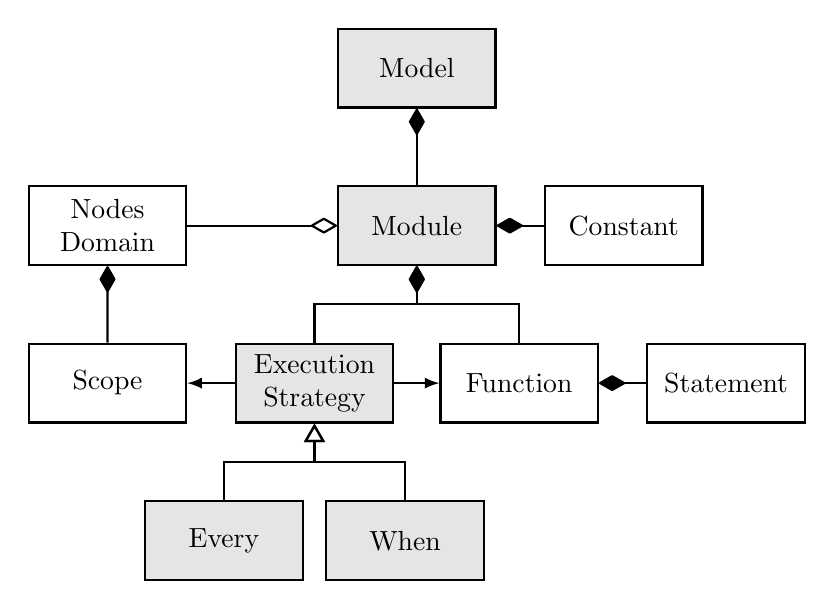
\begin{tikzpicture}[
  edge from parent fork down,
  sibling distance=5mm, level distance=20mm, node distance=6mm
  ]
  \node (model) [class,fill=black!10!white] {Model}
      child {node (module) [class,fill=black!10!white] {Module} edge from parent [composite]
        child {node (strategy) [class,align=center,xshift=-10.5mm,fill=black!10!white] {Execution\\Strategy} edge from parent [composite]
          child {node(every) [class,xshift=-9mm,fill=black!10!white] {Every} edge from parent [subclass]}
          child {node (when) [class,xshift=9mm,fill=black!10!white] {When} edge from parent [subclass]}
        }
        child {node (function) [class,xshift=10.5mm] {Function} edge from parent [composite]}
      };
  \node (constant)  [class,right=of module]   {Constant};
  \node (scope)     [class,left=of strategy]  {Scope};
  \node (statement) [class,right=of function] {Statement};
  \node (nodes)     [class,left=of module,xshift=-13mm]    {Nodes\\Domain};
  
  \draw [aggregate]  (module)   -- (nodes);
  \draw [composite]  (module)   -- (constant);
  \draw [dependency] (strategy) -- (scope);
  \draw [composite]  (function) -- (statement);
  
  \draw [composite]  (nodes)    -- (scope);
  \draw [dependency] (strategy) -- (function);
\end{tikzpicture}
}
\caption{Partial Semantic Model for \NAME. Shaded classes indicate the \emph{event/scheduling} construction around functions to allow interpretation.}
\label{fig:meta-model}
\end{figure}

The concept driving this model is the structure starting at the \emph{Model} up
to the \emph{Execution Strategy}. This structure encompasses the
\emph{Function}s and underlying \emph{Statement}s and allows for interpretation
and fusion of the algorithms.

\subsubsection{Functional Code Fusion (FCF)}

Thanks to the functional description of events and the effects triggered by
them, the code generator is able to identify the same actions across different
algorithms. This way it is possible to extract the parsing of incoming
messages, group actions on the same sets of data or scheduled function
executions.

FCF typically looks for patterns in the semantic model and performs model
transformations to change these patterns to a more optimized organization. It
first performs semantic transformations on the semantic model itself and ends
then transforms the semantic model into a syntactic model, encoding the
semantics into technical syntax constructs.

\subsubsection{Syntactic Model}

The syntactic model is an AST for a virtual, expressive language. It contains
constructs and ideas found in different languages and programming paradigms. No
single existing programming language supports all features as is. Syntactic
transformations therefore morph the unsupported constructs into comparable
constructs supported by the targeted platform and language.

Depending on the target platform, some constructions aren't transformed into
actually corresponding code. In selected cases, the generator uses a software
library. For example when it needs to parse incoming messages or schedule
tasks. During the generation process, it looks for patterns that indicate any
of these actions and transforms them into calls to the \NAME software library.

\subsection{\NAME as a Software Library}
\label{software-lib-design}

Section \ref{pattern-problems} introduced the option to use a software library
to offload common implementation aspects, thus avoiding small discrepancies in
code and suboptimal use of shared resources. Section \ref{dsl-unified-msg}
illustrated this approach with a case for unified messaging: parsing of
incoming messages and grouping of outgoing messages.

Other common functionality also isn't fully generated. The execution of
functions based on a schedule or the implementation of higher level conceptual
functions, such as \ttt{now} and \ttt{sha1}, are calls into the standard
software library that supports the code generator.

Optimizing such algorithms is not within the scope of \NAME. It also gives
freedom of choice to the users of the framework to select appropriate
implementations for this standard functionality.

\subsection{\NAME as a Framework}

\NAME reduces inefficiencies in execution, memory usage and network access, due
to the selection of separate ID algorithms. To achieve this, it avoids
constructions that are hard to identify and reorganize, such as loops and
common data. A DSL, focussing on event-handling, enforces these restrictions
and enables formally describing ID algorithms.

The DSL is also platform and language independent. This allows the source code
generator to target different configurations without any change to the formal
descriptions of the algorithms.

A supporting software library allows separation of standard functionality that
is out of scope for the generator. Optimization of the implementation of this
library for the specific platform and target language is possible.

\section{Implementation and Evaluation}
\label{evaluation}

This section discusses a prototype implementation and evaluates its
performance. We first present the architecture of this implementation and
consider the impact it has from a development point of view. Next we use this
implementation to quantify its merits using a side-by-side comparison of
generated code versus a manual implementation.

\subsection{Architecture}

Figure \ref{fig:architecture} shows the architecture of the implementation. It
illustrates the generation of the DSL into compilable code, using the Nodes
domain information, a platform and language description and the native software
library. The applied grayscale indicates the components' platform dependency:
the DSL is platform and language independent and deals with subsystems, such as
the network, in an abstract way. The Nodes domain implements some of these
abstracted subsystems, but still in a platform and language independent way.
The platform and language descriptions define the target platform and language
and convert the abstract constructions in actually supported code. The software
library is standard native code, targeting the platform and language. Finally,
the code and image are artifacts of the automated generation and compilation
process. They aren't a product of manual work and therefore aren't directly
dependent on the platform.

\begin{figure}[ht]
  \centering
  \scalebox{.85}{
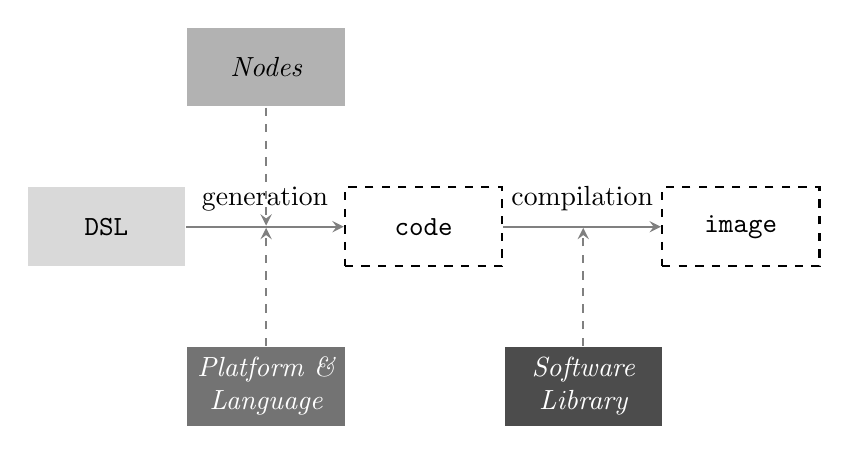
\begin{tikzpicture}[
  node distance=10mm and 20mm,
  ,>=stealth,thick,black!50,text=black,
  every new ->/.style={shorten >=1pt},
]
  \node (dsl)      [user,align=center]                                     {DSL};
  \node (code)     [generated,right=of dsl]                                {code};
  \node (image)    [generated,right=of code]                               {image};

  \node (nodes)    [dom,above right=of dsl,xshift=-20mm]                   {Nodes};
  \node (platform) [platform,below right=of dsl,align=center,xshift=-20mm] {Platform \&\\Language};
  \node (lib)      [native,below right=of code,align=center,xshift=-20mm]  {Software\\Library};

  \draw [->] (dsl)  -> (code)  node [midway,above=2pt] {generation};
  \draw [->] (code) -> (image) node [midway,above=2pt] {compilation};

  \draw [->,dashed] (nodes.south)    -> ++(0,-15mm);
  \draw [->,dashed] (platform.north) -> ++(0,15mm);
  \draw [->,dashed] (lib.north)      -> ++(0,15mm);
\end{tikzpicture}
}
  \caption{Architecture of Prototype Implementation}
  \label{fig:architecture}
\end{figure}

This hierarchy is important from a development effort point of view. The level
of dependency on the targeted platform also dictates the level of effort to
implement changes to that platform. For example: to generate a different
language will require a complete rewrite of the software library and a partial
rewrite of the language description of the generator. Although this is a
reusable, one-time effort, it is important in relation to the scalability of
the framework itself.

\subsection{Implementation}

To evaluate the prototype we chose to use a system based on the Atmel
ATMEGA1284p micro-controller \cite{datasheet:atmega1284p} and the Digi XBee S2
ZigBee module \cite{manual:xbee}. A basic library wrapped the technical calls
to the hardware components in more easy to use functions.

Relying on basic hardware and software allows us to validate that the generator
is capable of generating code even for the most basic environment available.
Any step up, both in hardware or software, would offer better and higher
abstractions that would make it easier to generate code for that situation. It
shows that the requirements of the generator towards the platform are minimal,
don't rely on advanced frameworks or operating systems and therefore are
applicable in any environment, targeting any platform.

For the evaluation we constructed a small meshed network. In this network, not
all devices have direct access to one another, requiring routing through shared
neighboring devices.

We started from a basic application that measures light intensity. The
application was an includable piece of code, which allowed integration in a
manual implementation and simple merging when generation. On top of this
baseline we added two intrusion detection related algorithms: a
watchdog \cite{mishra2004intrusion}, that allows nodes to validate each other's
presence, and a reputation-based algorithm \cite{ganeriwal2008reputation}, that
checks if a parent node is cooperative and actually forwards messages further
upstream.

\subsection{Experimental Results}

We evaluated three criteria: the image size of the resulting compiled code, the
network usage in number of frames and bytes and the time required to perform
once cycle of the event loop. To do this, we collected these metrics for four
situations: without ID algorithms, with a watchdog, with reputation-tracking
and with both algorithms implemented.

The manual implementation implemented both algorithms as standalone modules and
sequentially called them from the base-application's event loop. Given the
\NAME descriptions of the algorithms, the code generator generated all four
cases.

Tables \ref{tbl:manual} and \ref{tbl:generated} show the collected data for the
manual and the generated implementation. They present the base case in absolute
values and the implementations with the ID algorithms relative to that base
case.

\begin{table}[H]
  \centering
  \begin{tabular}{lrrrr}
  \hline
      & base & watchdog & reputation & both\\
  \hline
  size (bytes) & 10500 & 148\% & 127\% & 175\%\\
  frames & 20 & 255\% & 160\% & 315\%\\
  bytes & 476 & 406\% & 181\% & 487\%\\
  time ($\mu$s) & 48 & 196\% & 183\% & 310\%\\
  \hline
  \end{tabular}
  \caption{Results for the manual implementation.}
  \label{tbl:manual}
\end{table}

\begin{table}[H]
  \centering
  \begin{tabular}{lrrrr}
  \hline
         & base & watchdog & reputation & both\\
  \hline
  size (bytes) & 10496 & 175\% & 156\% & 200\%\\
  frames & 20 & 245\% & 160\% & 275\%\\
  bytes & 476 & 399\% & 186\% & 454\%\\
  time ($\mu$s) & 48 & 252\% & 252\% & 288\%\\
  \hline
  \end{tabular}
  \caption{Results for the generated implementation.}
  \label{tbl:generated}
\end{table}

These results show that adding algorithms manually to the base-application has
a cumulative effect. The impact of both algorithms is simply the sum of the
impact of each algorithm by itself. In case of the execution time of one cycle
of the event loop, the total is even a bit higher.

In case of the generated implementation, this effect is no longer observed:
individual algorithms do have a larger impact by themselves, but the
combination of both algorithms is less than the sum of both.

Most remarkable is the effect on the time of one event loop cycle: both
algorithms by itself add 152\%. Adding a second algorithm only augments the
impact to 188\%. We see the effect of the generic handling of common
functionality, like message parsing, event scheduling,\dots It comes with an
overhead for a single algorithm, but pays for itself when adding more
algorithms.

Table \ref{tbl:summary} compares the two situations by subtracting the manual
case from the generated case, showing the impact of the code generation. A
relative value for the entire implementation with both algorithms is also
presented.

\begin{table}[H]
  \centering
  \begin{tabular}{lrrrrr}
  \hline
                & base & watchdog & reputation & both  & result \\
  \hline
  size (bytes)  & -4    & 2822     & 3070       & 2664  & 115\%  \\
  frames        & 0     & -2       & 0          & -8    & 87\%   \\
  bytes         & 0     & -36      & 24         & -156  & 93\%   \\
  time ($\mu$s) & 0     & 27       & 33         & -11   & 93\%   \\
  \hline
  \end{tabular}
  \caption{Comparison of both manual and generated implementations.}
  \label{tbl:summary}
\end{table}

The first observation deals with the base case: both the manual and the
generated implementations perform exactly the same. There is no fundamental
structural difference in the overall architecture of the code.

Secondly, we see that the software library that comes with the generated code
adds to the size of the resulting image. But the cost is close to constant and
is lower for both algorithms together. With roughly 3KB of additional overhead,
or 15\% in this simple case, this impact limited.

Thirdly, when turning to the goal to reduce the network usage, we see that both
the number of frames as well as the amount of bytes sent have dropped by 13 and
7\%.

Finally we see that both algorithms by itself add an equal amount of time to
the processing of a single event loop cycle, but when combined, the event loop
is about 7\% faster compared to the manual case.

\section{Related Work}
\label{related}

Section \ref{classification} introduced some ID
algorithms \cite{ganeriwal2008reputation,mishra2004intrusion,krontiris2009cooperative}
and presented a classification \cite{mishra2004intrusion,ioannis2007towards,alrajeh2013intrusion}
based on their detection approach and interaction style.

This section focuses on related work in the field of domain specific languages
and code generation, both in relation to wireless networks of resource
constraint devices. These two components are the core of the \NAME framework
and the solution it proposes. We also look at the more general scope: the
application in other disciplines and their relevance in the scope of intrusion
detection in the IoT and the proposed \NAME framework.

\subsection{Domain Specific Languages}

Within the scope of wireless networks of resource constraint devices, we see
the introduction of DSLs \enquote{to shorten the development cycles
dramatically during deployments, to reduce the dependency on hardware and
software engineers, and to lead to a wider adoption outside the computer
science field} \cite{sadilek2008domain,naumowicz2009prototyping}.

TinyScript \cite{levis2004tinyscript} is an example of a language for wireless
sensor networks. It's a complete programing language that aims to ease the
description of algorithms in general. The Basic-like syntax does enable more
productive development. But this approach doesn't address the underlying
resource problems inherently connected to the context.

SEAL \cite{elsts2013seal} is a novel complete programming language that focuses
on novice programmers. It is a clear fit for \emph{sense-and-send} type of
applications, and doesn't pretend to be the best choice for any type of
application. It does however share the idea of event to overcome the technical
nature of loops.

Shifting the scope to intrusion detection, we learn that DSLs are predominantly
used to describe patterns of events found in network
packets \cite{sekar1999high,roesch1999snort} in a concise way.

BMSL \cite{uppuluri2001experiences} is a DSL that allows the specification of
patterns and actions. Patterns can contain events extracted from log files,
system calls and network packets.

The STAT framework with its STATL
language \cite{eckmann2002statl,vigna2003designing} are not intrusion detection
specific, but through extensions they allow to model attack scenarios using
state machines. Our event-driven approach shares this same ideas.

\subsection{Code Generation}

Code generation, in combination with a DSL, can optimize a development process
by reducing the size of the code base or systematically improving the code
quality.

Embedded systems are a prime example of an environment where code needs to be
of a high quality. Focus on size and performance are a logical choice when
dealing with limited storage and processing power. Compilers implement
different techniques to address this at the lowest level \cite{leupers2000code,
marwedel2002code}.

Optimizing for power efficiency however proves to be concurrent to size and
performance optimization, and requires different strategies. Data and memory
optimizations \cite{panda2001data} can result in improvements on a lower level.
But really preserving energy requires higher-level strategies, targeting
architecture, radio handling, efficient software,\dots \cite{naik2001software}.
Most of these are beyond the control of the compiler and require a higher level
of abstraction to address them.

DSLs are a solution here, but other paradigms are possible. A mixed framework
consisting of a virtual machine (VM) and native code
extension \cite{sadilek2007energy}, combined with energy-aware compilation,
seems a promising approach. By offloading the optimization to a VM and only
compiling parts and not the whole, the solution allows updating at a granular
scale, thus reducing the update cost, while maintaining flexibility and
lowering the development effort. As explained in \ref{positioning}, \NAME
focuses on the reduction of the development effort and update cost, while
preserving flexibility.

Finally, applying code generation to IDS, typically tries to generate native
code to avoid the interpretation of the description of patterns.
I2S \cite{charitakis2003code} is an example that generates code for
SNORT \cite{roesch1999snort} rules. To optimize this highly efficient code, it
often targets a specific platform.

\section{Conclusion and Future Work}
\label{conclusion}

Adequate intrusion detection for IoT devices requires multiple algorithms to
operate at the same time. Recent literature describes different algorithms, but
hardly any are readily available for direct application when implementing an
IDS for IoT devices. Reselection of algorithms, due to changing requirements or
security threats, requires a flexible way to incorporate the different
algorithms. This eliminates manual implementation and optimization.

Wireless resource constraint devices, such as IoT devices, require that
software respects their restrictions. Efficiently adding multiple intrusion
detection algorithm requires fusion of these algorithms on a functional level,
to reduce execution inefficiencies, redundant memory usage and superfluous
network access.

\NAME is a framework consisting of a DSL, a source code generator and
accompanying software library. Using the DSL, intrusion detection algorithms
can be formally described in terms of functionality. During source code
generation, functional code fusion interprets the functional meaning of the
algorithms and merges common functionality and shared data. The software
library hosts common functionality, such as network message parsing, sent
message aggregation, event scheduling,\dots This allows the source code
generator to focus on the optimization of the organization of the functionality.

Initial experiments confirm the theoretical positive impact on resource usage.
The platform independent DSL enables generation of source code targeting
different platforms and languages, which allows high degrees of reuse in
heterogenous environments and different configurations.

Future research will focus on the integration of applications with the
generated intrusion detection systems. We see opportunities for applications
who detect intrusion, to actively and dynamically respond and avoid malicious
payloads to harm them.

A continued effort is targeting the reduction of non-platform independent parts
in the implementation. This way it is possible to add more platforms and
languages with less effort.

In the longer run, we want to investigate the possibility to extend the
functional code fusion paradigm to other domains beyond intrusion detection.

\section{Acknowledgements}

This research is partially funded by the Interuniversity Attraction Poles
Programme Belgian State, Belgian Science Policy, and by the Research Fund KU
Leuven. This research is partially funded by the EU FP7 project NESSoS\@. We
would like to thank the reviewers for their thoughtful and helpful comments
that enhanced the readability of this paper.

\bibliographystyle{IEEEtran}
\bibliography{literature/referenties}

\end{document}
